\documentclass[11pt,a4paper]{book}
\usepackage[brazilian]{babel}
\usepackage[utf8]{inputenc}
\usepackage[T1]{fontenc}
\usepackage[inline]{enumitem}
\usepackage{xcolor}
\usepackage{listings}
\usepackage{graphicx}
\usepackage{multicol}
\usepackage{amsmath}

\definecolor{mGreen}{rgb}{0,0.6,0}
\definecolor{mGray}{rgb}{0.5,0.5,0.5}
\definecolor{mPurple}{rgb}{0.58,0,0.82}
\definecolor{backgroundColour}{rgb}{0.95,0.95,0.92}

\lstdefinestyle{CStyle}{
    backgroundcolor=\color{backgroundColour},   
    commentstyle=\color{mGreen},
    keywordstyle=\textbf{\color{black}},
    numberstyle=\tiny\color{mGray},
    stringstyle=\color{mPurple},
    basicstyle=\footnotesize,
    breakatwhitespace=false,         
    breaklines=true,                 
    captionpos=b,                    
    keepspaces=true,                 
    numbers=left,                    
    numbersep=5pt,                  
    showspaces=false,                
    showstringspaces=false,
    showtabs=false,                  
    tabsize=2,
    frame=single,
    escapeinside={(*}{*)},
    language=C
}

\makeatletter
% This command ignores the optional argument for itemize and enumerate lists
\newcommand{\inlineitem}[1][]{%
\ifnum\enit@type=\tw@
    {\descriptionlabel{#1}}
  \hspace{\labelsep}
\else
  \ifnum\enit@type=\z@
       \refstepcounter{\@listctr}\fi
    \quad\@itemlabel\hspace{\labelsep}
\fi}
\makeatother

\newcommand{\onestaritem}{\refstepcounter{enumi}\item[$*$\theenumi.]}
\newcommand{\twostaritem}{\refstepcounter{enumi}\item[$**$\theenumi.]}

\title{Lista 5: Fundamentos Estatísticos para Ciência dos Dados}
\author{Ricardo Pagoto Marinho}

\begin{document}
\maketitle
	\begin{enumerate}
		\item

			O código e os dados estão em https://github.com/ricardopmarinho/UFMG/tree/master/Mat%C3%A9rias/FECC/Lista%205
		
			O problema proposto consiste em olhar o perfil de tráfego em uma rede Wi-Fi durante a utilização do site \textit{Facebook}.
			Desta forma, olharei para o protocolo utilizado em cada pacote, \textit{i.e.}, TCP, UDP, DNS, ARP, etc.
			Além disto verificarei o tamanho de cada pacote.
			Para isso, utilizarei o programa \textit{Wireshark}, que captura todos os pacotes que estão passando (tanto de entrada como de saída) em uma interface do computador analisado.
			Dentre os vários protocolos que possivelmente são utilizados em uma rede, os da camada de transporte tentem a se repetir mais vezes, já que usualmente são utilizados apenas dois: TCP e UDP, enquanto que nas outras, a quantidade de protocolos pode variar mais.
			Além disso, olharei o tamanho dos pacotes em bytes.
			O site é acessado antes de começar o monitoramento, logo, os pacotes maiores, que contem as imagens e dados do site, não serão capturados.
			
			\begin{itemize}
				\item Protocolos
			
					Foram identificados 13 protocolos no teste com as seguintes frequências:
					\begin{tabular}{|c|c|}
						\hline
						Protocolo & Frequência\\
						\hline
						ARP & 2\\
						\hline
						DB-LSP-DISC & 8\\
						\hline
						DHCPv6 & 1\\
						\hline
						DNS & 4\\
						\hline
						ICMP & 4\\
						\hline
						LLMNR & 4\\
						\hline
						MDNS & 2\\
						\hline
						NBNS & 3\\
						\hline
						QUIC & 20\\
						\hline
						SSL & 5\\
						\hline
						TCP & 28\\
						\hline
						TLSv1.2 &  17\\
						\hline
						UDP & 2\\
						\hline
					\end{tabular}
					Considerando a distribuição dos dados como uma Poisson com $\lambda=5$ pois é sabido que a chegada de pacotes em uma rede segue essa distrubuição e dividindo os protocolos em grupos de 2 (com exceção do UDP, que ficou sozinho), os conjuntos de protocolos e suas frequências foram:
					\begin{tabular}{|c|c|}
						\hline
						Protocolos & Frequência\\
						\hline
						ARP\& DB-LSP-DISC & 10\\
						\hline
						DHCPv6\& DNS & 5\\
						\hline
						ICMP\& LLMNR & 8\\
						\hline
						MDNS\& NBNS & 5\\
						\hline
						QUIC\& SSL & 25\\
						\hline
						TCP\& TLSv1.2 & 45\\
						\hline
						UDP & 2\\
						\hline
					\end{tabular}
					Utilizando a distribuição de Poisson com a configuração dita, os valores esperados foram:
					
					\begin{tabular}{|c|c|}
						\hline
						Protocolos & Frequência\\
						\hline
						ARP\& DB-LSP-DISC & 12.4\\
						\hline
						DHCPv6\& DNS & 40.6\\
						\hline
						ICMP\& LLMNR & 49.7\\
						\hline
						MDNS\& NBNS & 31.5\\
						\hline
						QUIC\& SSL & 11.9\\
						\hline
						TCP\& TLSv1.2 & 2.9\\
						\hline
						UDP & 0.5\\
						\hline
					\end{tabular}
										
					A Figura~\ref{fig:fig1}, mostra a distribuição em relação aos protocolos.
					
					\begin{figure}[t]
						\centering
						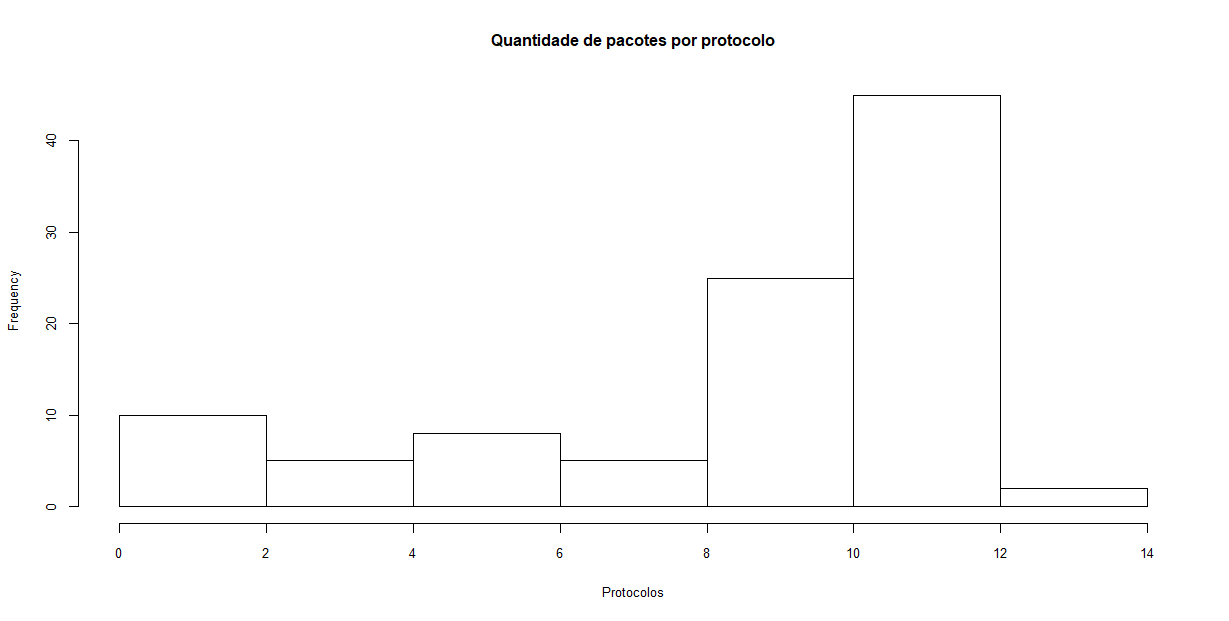
\includegraphics[height=5cm]{prot.png}
						\label{fig:fig1}
						\caption{Protocolos}
					\end{figure}
					
				\item Tamanho dos pacotes
					Para o tamanho dos pacotes, foram divididos em 14 grupos, variando de 0 a 1400 bytes, ou seja, cada grupo é uma janela de 100 bytes.
					Suas frequências foram: 
					\begin{tabular}{|c|c|}
						\hline
						Janela & Frequência\\
						\hline
						[0,100] & 70\\
						\hline
						(100,200] & 7\\
						\hline
						(200,300] & 9\\
						\hline
						(300,400] & 5\\
						\hline
						(400,500] & 0\\
						\hline
						(500,600] & 2\\
						\hline
						(600,700] & 0\\
						\hline
						(700,800] & 0\\
						\hline
						(800,900] & 0\\
						\hline
						(900,1000] & 0\\
						\hline
						(1000,1100] & 0\\
						\hline
						(1100,1200] & 0\\
						\hline
						(1200,1300] & 0\\
						\hline
						(1300,1400] & 7\\
						\hline
					\end{tabular}
					
					Utilizando a distribuição de Poisson com $\lambda=50$, os valores esperados foram:
					\begin{tabular}{|c|c|}
						\hline
						Janela & Frequência\\
						\hline
						[0,100] & 100\\
						\hline
						(100,200] & 3x10$^{-8}$\\
						\hline
						(200,300] & 0\\
						\hline
						(300,400] & 0\\
						\hline
						(400,500] & 0\\
						\hline
						(500,600] & 0\\
						\hline
						(600,700] & 0\\
						\hline
						(700,800] & 0\\
						\hline
						(800,900] & 0\\
						\hline
						(900,1000] & 0\\
						\hline
						(1000,1100] & 0\\
						\hline
						(1100,1200] & 0\\
						\hline
						(1200,1300] & 0\\
						\hline
						(1300,1400] & 0\\
						\hline
					\end{tabular}

					A Figura~\ref{fig:fig2} mostra a distribuição das frequências dos tamanhos dos protocolos.
					
					\begin{figure}[t]
						\centering
						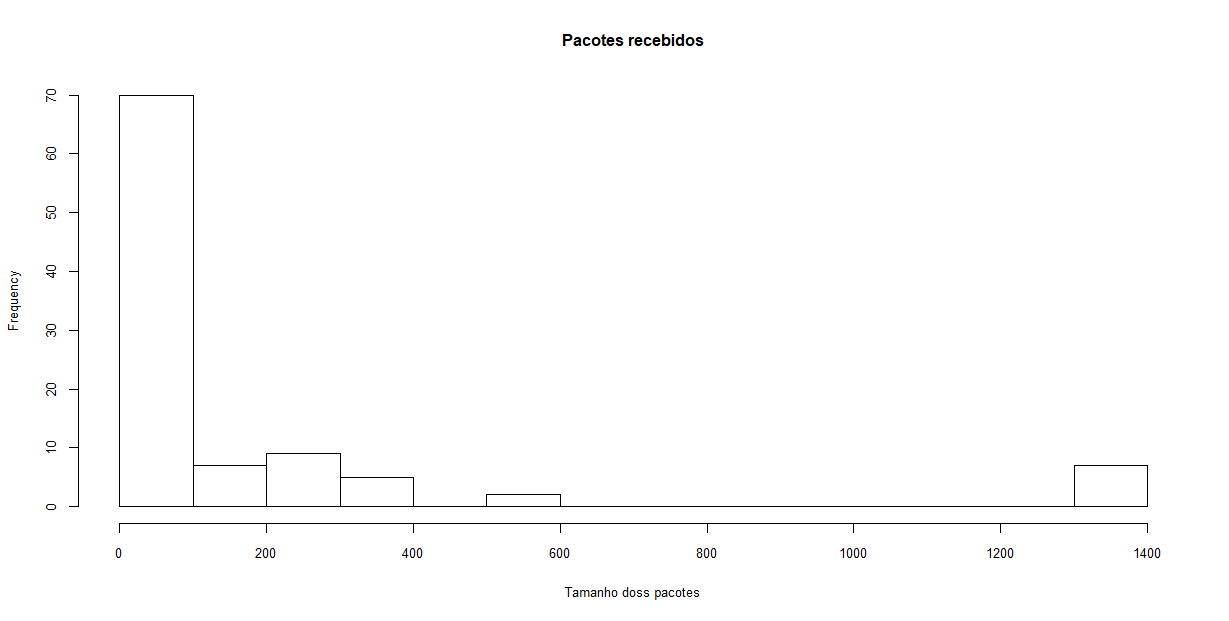
\includegraphics[height=5cm]{len.png}
						\label{fig:fig2}
						\caption{Tamanho dos pacotes}
					\end{figure}					
					
					Olhando para as figuras e para os resultados, podemos concluir que a distribuição utilizada não foi a mais adequada, fazendo que um olhar melhor sobre o tema se faça necessário.
			\end{itemize}
		\item
			\begin{itemize}
				\item 4.3-a) 0.6666667
				\item 4.3-b) 0.0625
				\item 4.3-c) 0.1428
				\item 4.14-a) cdf=$sum_{x=0}^{1} 20x^{3}\times~(1-x)$
				\begin{figure}[b]
					\centering
					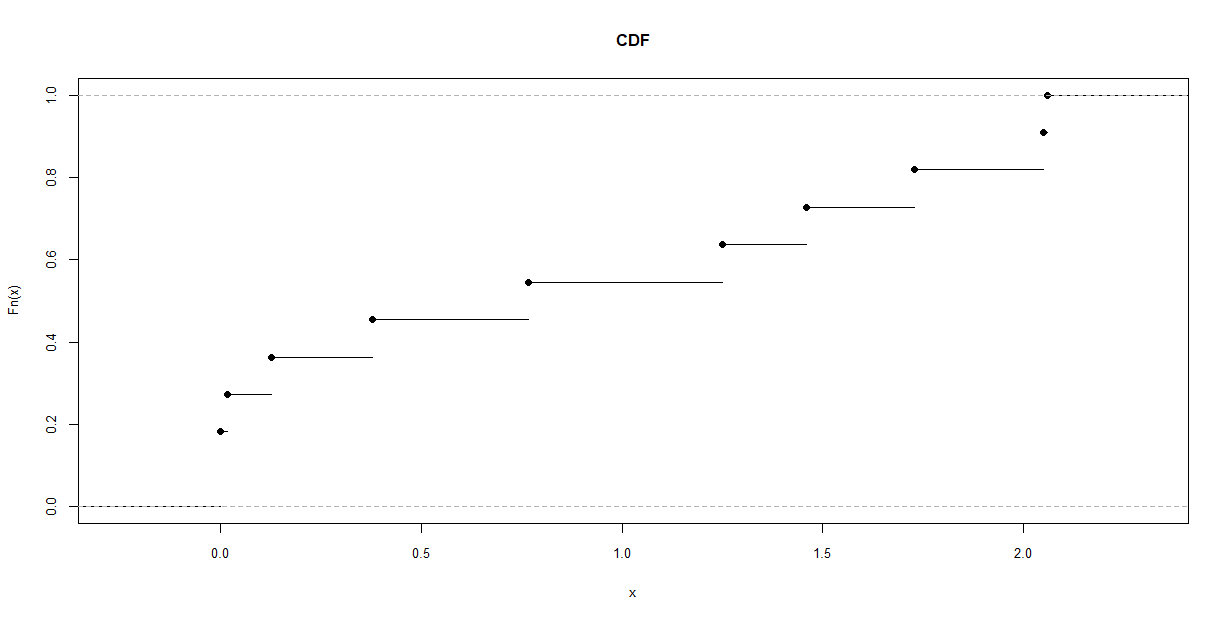
\includegraphics[height=6cm]{cdf.png}
					\label{fig:cdf}
					\caption{CDF}
				\end{figure}
				\item 4.14-b) Olhando a Figura~\ref{fig:cdf}, $P(X\leq~\frac{2}{3})=0.5$
			\end{itemize}
		\item
			\begin{itemize}
				\item
					\begin{figure}[b]
						\centering
						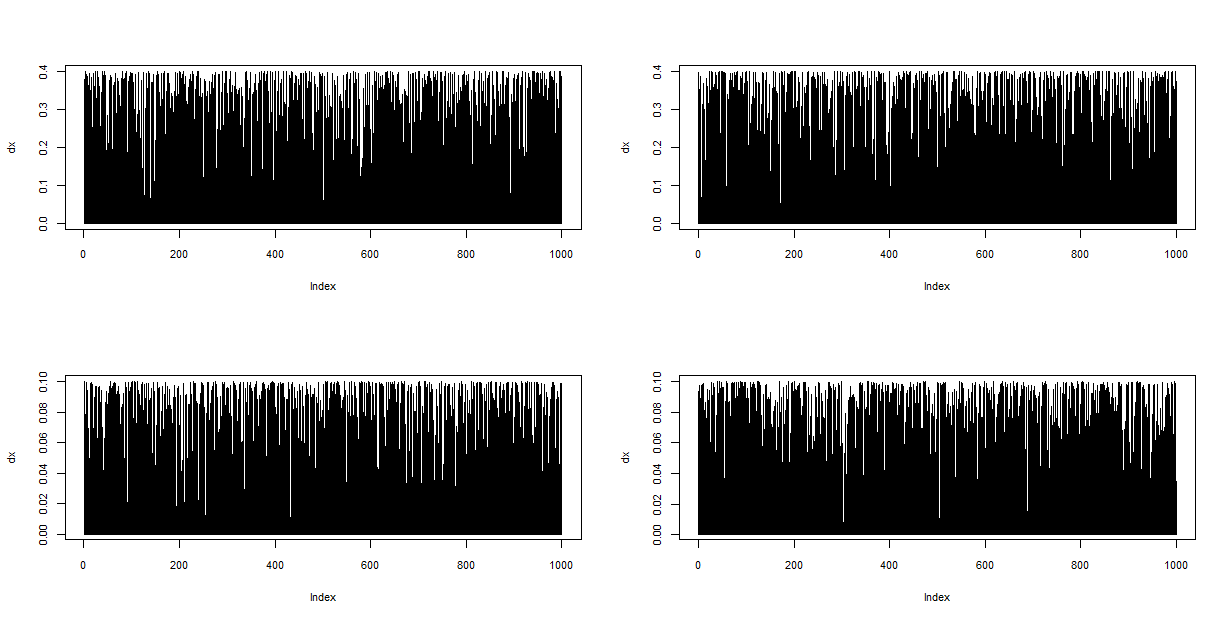
\includegraphics[height=6cm]{norm.png}
						\caption{Distribuição normal}
					\end{figure}
				\item o ponto em que f(x) assume o valor máximo varia, logo depende de $\delta$. A altura também depende. 
				\item
					pnorm(10+2*sqrt(5),10,5)-pnorm(10-2*sqrt(5)-0.01,10,5)
				
					0.629441
				\item
					\begin{figure}[t]
						\centering
						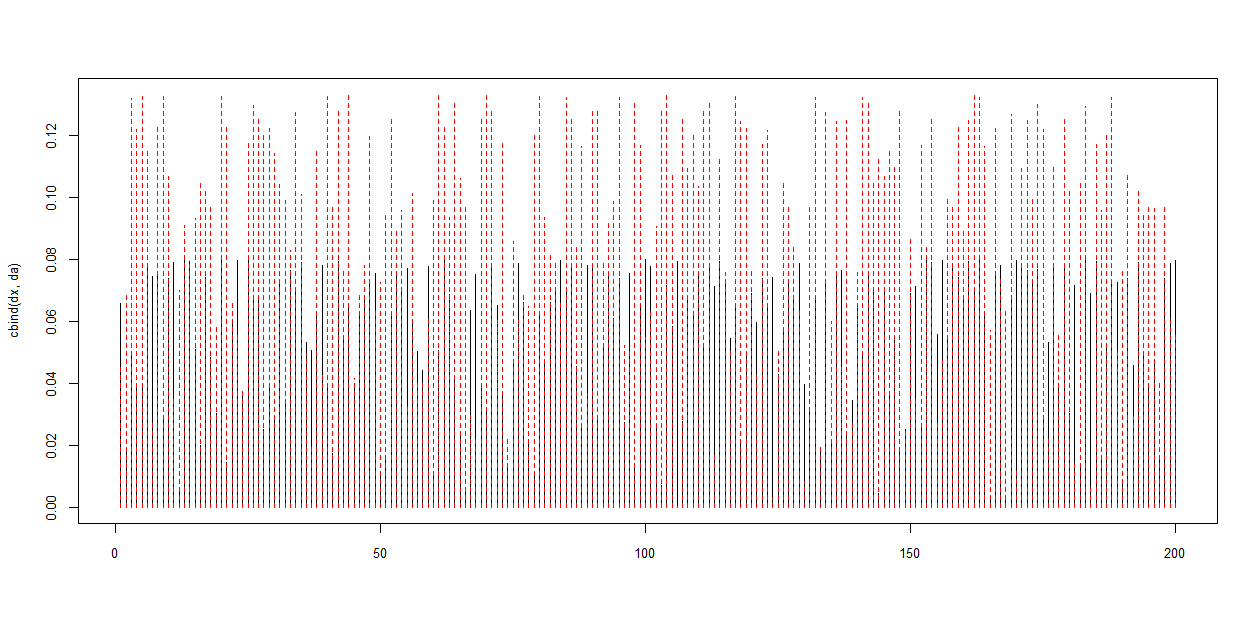
\includegraphics[height=6cm]{cbind.png}
						\caption{Sobreposição}
					\end{figure}
					
					Utilizei a configuração N(2,3).
					As distribuições se parecem sim, a altura que difere.
			\end{itemize}
		\item
			Todos os valores são iguais a 0.87297962.
			Nenhum valor ficou menor do que 0.05
		\item
			$E(X)=\frac{1}{\lambda}=\frac{1}{1/3}=3$
			
	\end{enumerate}
\end{document}